\documentclass[a4paper,10pt]{article}
\usepackage{a4wide}
\usepackage[T1]{fontenc}
\usepackage[utf8]{inputenc}
\usepackage[english]{babel}

\usepackage{xfrac} 				% gives \sfrac
\usepackage{amsmath}
\usepackage{enumerate} 		% allows you to change counters
\usepackage{verbatim}
\usepackage{comment}				% gives comment environment
\usepackage{hyperref}
\usepackage{amssymb}				% gives f.x. \mathbb{R}

% graphics packages
\usepackage{graphicx}
\usepackage{caption} 	
\usepackage{subcaption}
\usepackage{float}

\title{
	Assignment 2 - Basic Learning Algorithms	\\
	Statistical Methods for Machine Learning
  }
\author{
	Guðmundur Páll Kjartansson \\
	Jón Gísli Egilsson
}

% Uncomment to set paragraph indentation to 0 points, and skips a line
% after an ended paragraph.
\setlength{\parindent}{0pt}
\setlength{\parskip}{\baselineskip}

\begin{document}
\maketitle

\section*{II.1 Regression}

\subsection*{II.1.1 Maximum likelihood solution}

The models for variable selections $1$ and $2$ are implemented in the file \verb=regression.py=. We then applied both models to the test set and computed the RMS averaged over $100$ different selections of training and test data (where the training data was always $80\%$ and test data $20\%$ of the data in the file \verb=bodyfat.txt=). Our measured RMS errors for selection $1$ and $2$ respectively were
$$\text{RMS}_1 \approx 4.5$$
and
$$\text{RMS}_2 \approx 5.$$

\subsection*{II.1.2 Maximum a posteriori solution}

We also implemented the MAP estimate in \verb=regression.py=. In figure $1$ we can see the RMS error for the MAP estimate plotted for different values of the precision parameter $\alpha$. The RMS for the maximum likelihood solution was included in the plot for the same dataset for comparison.

Comparing the selections we see that selection $1$ seems to provide better prediction than selection $2$ given the minimizing $\alpha$ value. And if we chose $\alpha$ to be anywhere between $0$ and $0.1$ (not including $0$) we will get better results with the MAP estimate than the ML one. Similarly if we have $0 < \alpha \leq 0.24$ for selection $2$ the MAP provides better prediction than the ML one.

\begin{figure}[H]
	\centering
	\begin{subfigure}{0.45\textwidth}
  		\centering
  		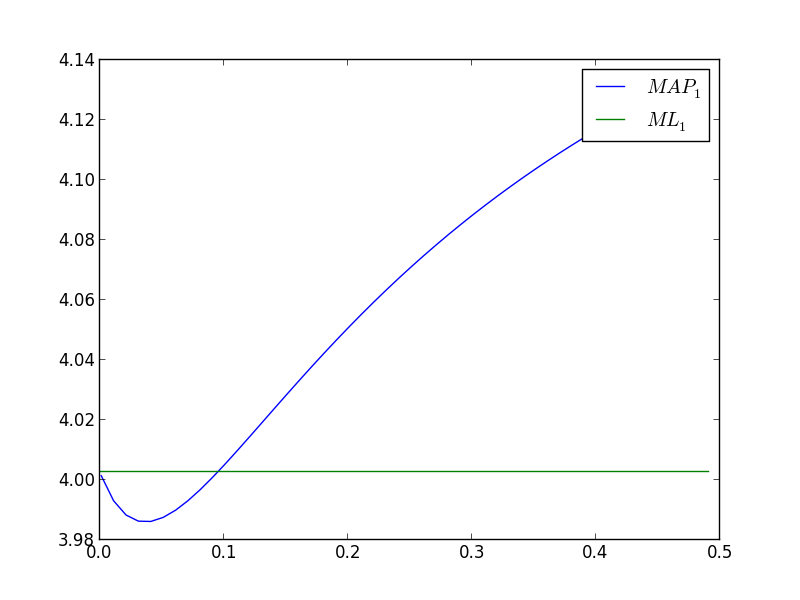
\includegraphics[width=\textwidth]{../images/report/rms_selection1.png}
  		\caption{Selection $1$}
  \end{subfigure}
  \begin{subfigure}{0.45\textwidth}
  		\centering
  		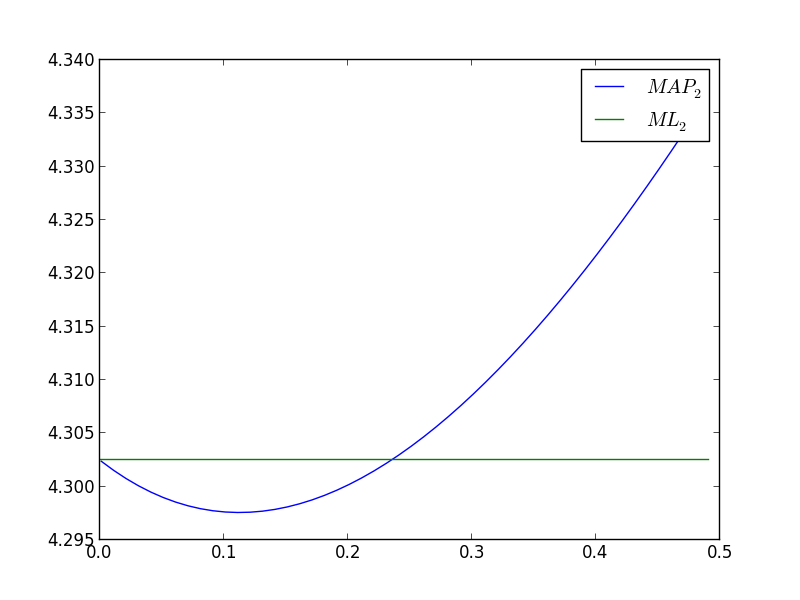
\includegraphics[width=\textwidth]{../images/report/rms_selection2.png}
  		\caption{Selection $2$}
  \end{subfigure}
  	\caption{RMS for MAP and ML}
\end{figure}

\subsection*{II.1.3 Maximum a posteriori solution}

We want to prove that 
$$p(w|t) = \mathcal{N}(w|m_N,S_N)$$
where
\begin{align*}
m_N &= S_N(S_0^{-1}m_0 + \beta \Phi^Tt) \\
S_N^{-1} &= S_0^{-1} + \beta \Phi^T \Phi.
\end{align*}
Now we see that
\begin{align*}
\ln(p(w|t)) &\propto \ln(p(w)p(t|w)) \\
		&= \ln(\mathcal{N}(w|m_0,S_0)) + \ln\left(\prod_{n=1}^N \mathcal{N}(t_n|w^T\phi(x_n),\beta^{-1})\right) \\
		&= -\frac{1}{2}(w-m_0)^T S_0^{-1} (w-m_0) + \sum_{n=1}^N \left( -\frac{1}{2}(t_n-w^T\phi(x_n))^T \beta (t_n-w^T\phi(x_n)) \right).
\end{align*}
Here we consider that $S_0^{-1} = \alpha I$ and $m_0 = 0$ we get by continuing from above that
\begin{align*}
\ln(p(w|t)) &\propto -\frac{1}{2}w^T \alpha I w + -\frac{1}{2}(t-\Phi w)^T \beta (t-\Phi w) \\
		&= -\frac{1}{2}\left( w^T \alpha I w + t^T\beta t - t^T \beta \Phi w - w^T\Phi^T \beta t + w^T \Phi^T \beta \Phi w \right) \\
		&\propto -\frac{1}{2}\left( w^T (\alpha I + \beta \Phi^T \Phi) w - \beta t^T  \Phi w - \beta w^T\Phi^T t \right) \\
		&= -\frac{1}{2}\left( w^T S_N^{-1} w - \beta t^T  \Phi w - \beta w^T\Phi^T t \right) \quad (\ast).
\end{align*}
Now we will note that 
\begin{align*}
\ln(\mathcal{N}(w|m_N,S_N)) &= -\frac{1}{2} (w - S_N(S_0^{-1}m_0 + \beta \Phi^Tt))^T S_N^{-1}(w - S_N(S_0^{-1}m_0 + \beta \Phi^Tt)) \\
		&\propto -\frac{1}{2}\left( w^T S_N^{-1} w - \beta (S_N\Phi^T t)^T S_N^{-1} w - \beta w^T S_N^{-1} S_N \Phi^T t \right) \\
		&= -\frac{1}{2}\left( w^T S_N^{-1} w - \beta t^T \Phi S_N^T S_N^{-1} w - \beta w^T S_N^{-1} S_N \Phi^T t \right)
\end{align*}
We know that $S_N$ is a symmetric matrix so $S_N^T = S_N$ and $S_N^T S_N^{-1} = I$. Then
$$\ln(\mathcal{N}(w|m_N,S_N)) \propto -\frac{1}{2}\left( w^T S_N^{-1} w - \beta t^T \Phi w - \beta w^T \Phi^T t \right)$$
which is the same result as we got in $(\ast)$. Thus we have shown that
$$p(w|t) = \mathcal{N}(w|m_N,S_N).$$


\section*{II.2 Classification}

\subsection*{II.2.1 Linear discriminant analysis}

We implemented the linear discriminant analysis algorithm in \verb=classification.py=. In figure $2$ we can see the three different classes in the training data.
\begin{figure}[H]
	\centering
  		\centering
  		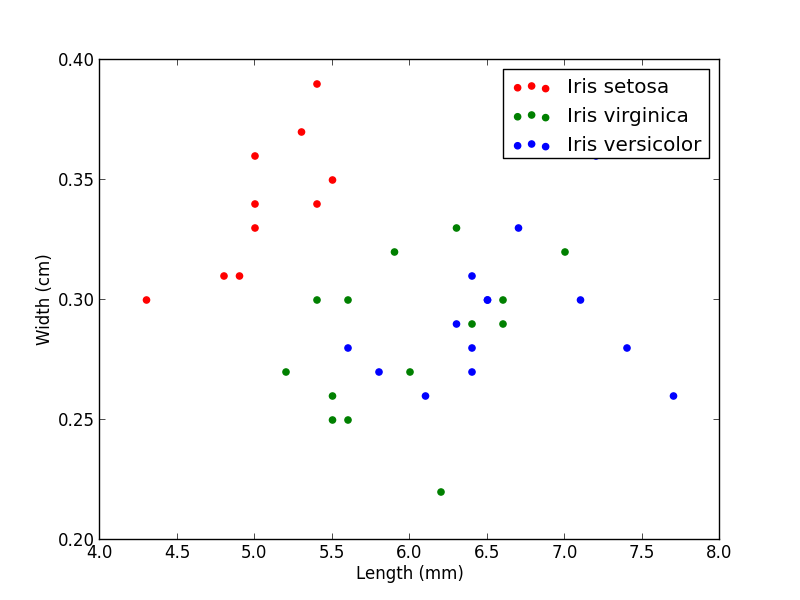
\includegraphics[width=0.6\textwidth]{../images/report/iris_scatter.png}
  		\caption{Scatter plot of Iris data}
\end{figure}
Now to quantify the error of the LDA we compute the probability of misclassification for the training and test data respectively. The errors are
$$\epsilon_{\text{training}} = 0.21$$
and
$$\epsilon_{\text{test}} = 0.18.$$

\subsection*{II.2.2 Nearest neighbour with Euclidean metric}

The $k$-nearest neighbour classifier is implemented in the file \verb=classification.py=, in a function called \verb=k_closest_norm=.

We train the function on the training dataset and then test its accuracy
on the training and test datasets for $k=1,3,5$ and $7$ neigbours.

Error on irisTrain:
\begin{center}
\begin{tabular}{l|llll}
 k & total error & class 0 & class 1 & class 2\\ \hline
 1 & 0.000000 & 0.000000 & 0.000000 & 0.000000\\
 3 & 0.289474 & 0.100000 & 0.357143 & 0.357143\\
 5 & 0.263158 & 0.000000 & 0.500000 & 0.214286\\
 7 & 0.315789 & 0.100000 & 0.571429 & 0.214286\\
\end{tabular}
\end{center}

Error with norm as a metric on irisTest:
\begin{center}
\begin{tabular}{l|llll}
 k & total error & class 0 & class 1 & class 2\\ \hline
 1 & 0.350000 & 0.138889 & 0.657143 & 0.241379\\
 3 & 0.270000 & 0.083333 & 0.400000 & 0.344828\\
 5 & 0.220000 & 0.083333 & 0.285714 & 0.310345\\
 7 & 0.230000 & 0.111111 & 0.371429 & 0.206897\\
\end{tabular}
\end{center}

We can see that the nearest neighbour model has perfect accuracy when
applied on its own training set with respect to one neighbour. The reason
is that every point we classify will be classified based on itself from
the original dataset. The error tends to increase if we increase the number of
neighbours beyond k=1, since some points have close neighbours belonging to another class (this is especially true for class 1 and 2 since they have a lot of overlap).

When the probability model from the training set is applied on the test set,
the most accurate value for k appears to be 5. The case when $k=1$ is worst
of the tested values, since the closest neighbour of a given point is not
so likely to belong to the same class.

\subsection*{II.2.3 Changing the metric}

Since $M$ is non-singular, we have that for any vector $x$ there is a unique $y$ such that $Mx=y$ and vice versa. This will be used in our proofs.\\

\subsubsection*{Proof that d is non decreasing}
\[
d(x,y)=||Mx-My||\geq0
\]
Trivial, since euclidean-norm is non-decreasing by definition.\\

\subsubsection*{Proof that $d(x,y) \iff x=y$}
Proof that $d(x,y)=0 \Rightarrow x=y$:
\begin{align*}
d(x,y)&=0\\
||Mx-Mz||&=0\\
x'-z'&=0, \text{where }Mx=x', Mz=z'\\
x'&=z'\\
x&=z
\end{align*}

Proof that $x=y => d(x,y)=0$:
\begin{align*}
x&=y\\
x-y&=0\\
Mx-My&=0\\
||Mx-My||&=0\\
d(x,y)&=0
\end{align*}
\subsubsection*{Proof of symmetry $d(x,y)=d(y,x)$}
By contradiction:
\begin{align*}
&d(x,y)\neq d(y,x)\\
\Rightarrow &||Mx-My||\neq ||My-Mx||\\
\Rightarrow &||c||\neq ||-c||, \text{where } c= Mx-My\\
\end{align*}
Which contradicts the euclidean-norm.
\subsubsection*{Proof of triangular inequality}
\begin{align*}
d(x,z) &\leq d(x,y) + d(y,z)\\
||Mx-Mz|| &\leq ||Mx-My|| + ||My-Mz||\\
||M(x-z)|| &\leq ||M(x-y)|| + ||M(y-z)||\\
\end{align*}
We know that:
\begin{align*}
||M(x-z)|| &= ||M(x-y) + M(y-z)||\\
           &= ||Mx-My+My-Mz||\\
	   &= ||Mx-Mz||
\end{align*}
We substitute in for $M(x-z)$:
\begin{align*}
||M(x-y) + M(y-z)|| &\leq ||M(x-y)|| + ||M(y-z)||\\
\end{align*}
Given $M(x-y)=a$ and $M(y-z)=b$:
\begin{align*}
||a + b|| &\leq ||a|| + ||b||\\
\end{align*}
Which holds for all vectors $a,b\in R^2$, according to
the triangular inequality.

\subsection*{II.2.4 Nearest neighbour with non-standard metric}

Now we will repeat the classification done in section II 2.2, except we will
use the metric given in II 2.3 on the dataset.

First we will try to classify \verb=irisTrain.dt= with a probability model based on the $d$ metric. The error of these results can be seen in the table below:

Error with $d$ as a metric on \verb=irisTrain.dt=:
\begin{center}
\begin{tabular}{l|llll}
 k & total error & class 0 & class 1 & class 2\\ \hline
 1 & 0.000000 & 0.000000 & 0.000000 & 0.000000\\
 3 & 0.236842 & 0.000000 & 0.285714 & 0.357143\\
 5 & 0.315789 & 0.100000 & 0.500000 & 0.285714\\
 7 & 0.289474 & 0.100000 & 0.500000 & 0.214286\\
\end{tabular}
\end{center}

As expected, $k=1$ is optimal here. We can see that the error for class $0$ is always very low, but it's higher for the other classes.

Error with d as a metric on \verb=irisTest.dt=:
\begin{center}
\begin{tabular}{l|llll}
 k & total error & class 0 & class 1 & class 2\\ \hline
 1 & 0.290000 & 0.083333 & 0.600000 & 0.172414\\
 3 & 0.310000 & 0.083333 & 0.342857 & 0.551724\\
 5 & 0.270000 & 0.083333 & 0.342857 & 0.413793\\
 7 & 0.230000 & 0.083333 & 0.342857 & 0.275862\\
\end{tabular}
\end{center}

Here we seem to misclassify the same amount of points for class $0$ at all times and for class $1$ at all times except when $k=1$.

These error values are different from those we got in II 2.2 when we
used the euclidian-norm.

\subsubsection*{Performance differences}
Difference in error between Norm and $d$ on \verb=irisTrain.dt=:\\
\begin{center}
\begin{tabular}{l|llll}
 k & total error & class 0 & class 1 & class 2\\ \hline
 1 & 0.000000 & 0.000000 & 0.000000 & 0.000000 \\
 3 & 0.052632 & 0.100000 & 0.071429 & 0.000000 \\
 5 & -0.052632 & -0.100000 & 0.000000 & -0.071429 \\
 7 & 0.026316 & 0.000000 & 0.071429 & 0.000000 \\
\end{tabular}
\end{center}

Difference in error between Norm and $d$ on \verb=irisTest.dt=:\\
\begin{center}
\begin{tabular}{l|llll}
 k & total error & class 0 & class 1 & class 2\\ \hline
 1 & 0.060000 & 0.055556 & 0.057143 & 0.068966 \\
 3 & -0.040000 & 0.000000 & 0.057143 & -0.206897 \\
 5 & -0.050000 & 0.000000 & -0.057143 & -0.103448 \\
 7 & 0.000000 & 0.027778 & 0.028571 & -0.068966 \\
\end{tabular}
\end{center}

A positive value means that the d metric is more precise and vice versa. The $d$ metric is apparently less precise for $k=3$ and $k=5$.
The reason for these differences is that when we look for the nearest
neighbours using the d metric, the y-axis is scaled by a factor of $10$. This means that neighbours to the left and right of a point will appear ten times
closer than neighbours above and below.



\subsection*{II.2.5 LDA with rescaled data}

The rescaled data with $M$ can be found in the files \verb=irisTrain.dt.scaled= and \verb=irisTest.dt.scaled=. The training and test errors we get for this transformed data are the same as we got before the transformation or 
$$\epsilon_{\text{training}} = 0.21$$
and
$$\epsilon_{\text{test}} = 0.18.$$
The short answer to \emph{why} we get the same errors is \emph{linearity}. This transformation by $M$ is just rescaling of the $y$-axis.


\begin{comment}
\begin{figure}[H]
	\centering
	\begin{subfigure}{0.45\textwidth}
  		\centering
  		\includegraphics[width=\textwidth]{../week4/images/prob41asurf.png}
  		\caption{$x=(0,-1)$}
  \end{subfigure}
  \begin{subfigure}{0.45\textwidth}
  		\centering
  		\includegraphics[width=\textwidth]{../week4/images/prob41bsurf.png}
  		\caption{$x=(0,0.05)$}
  \end{subfigure}
  	\caption{Surface plots of $m(p)$ at different points}
\end{figure}
\end{comment}


\end{document}




































